\subsection{Pipeline}

Um die im zuvor beschriebenen Kapitel möglichen Verteilungen zu realisieren, kann eine Pipeline aufgebaut werden, um diese Schritte abzuarbeiten. Dabei würde jeder Rechner Aufgaben aus einer Queue bekommen und diese an die Nächste Queue weiterschicken. Somit wäre eine gleichmäßige Verteilung der Aufgaben möglich und die Rechner sind voneinander entkoppelt. Die Entkopplung der Rechner ermöglicht außerdem die Verwendung von verschiedenen Programmiersprachen bei den unterschiedlichen Aufgaben. Um dies zu Realisieren benötigt es jedoch einen Rechner der als Initiator des Algorithmus wirkt und einen Rechner zum Einsammeln der Ergebnisse, der am Ende der Pipeline auf die Berechnung wartet.

\begin{figure}[h]
	\centering
	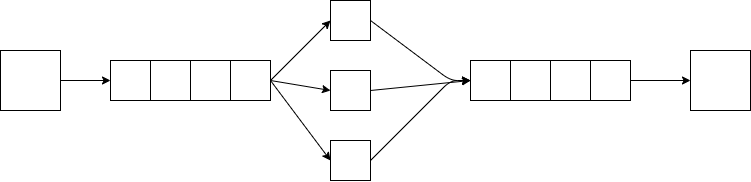
\includegraphics[width=0.5\textwidth]{queue.png}
	\caption{Beispiel der Pipeline}
	\label{pipeline}
\end{figure}